\chapter{Vizualizácie}
\todo[inline]{cd priloha/web, spustenie, requirements, ...}

Cieľom tejto práce je nielen popísať \obliv pamäťový model a rôzne dátové štruktúry v ňom, ale aj vytvoriť ich vizualizácie. Tie majú slúžiť na edukačné účely pre študentov (a učiteľov) a pomáhať pri pochopení ich fungovania.

\section{Software} \todo{softver? bleh...}
Výsledkom práce sú vizualizácie demonštrujúce dátové štruktúry popísané v predchádzajúcich sekciách: \vEB usporiadanie (sekcia \ref{sec:static-obliv}) v statickom binárnom vyhľadávacom strome, usporiadané pole (\ref{sec:orderedfile}) a dynamický b-strom (\ref{sec:dynamic-obliv}). Súčasťou je tiež simulácia \cache (sekcia \ref{sec:memmodel}) s možnosťou voľby parametrov $B$ a $M$ - veľkosť bloku a celková veľkosť.

Tieto vizualizácie sú implementované ako rozšírenie programu \emph{Gnarley trees}, ktorý vznikol ako súčasť bakalárskej práca Jakuba Kováča \citep{algviskuko}. Tento nástroj na vizualizáciu (prevažne stromových) dátových štruktúr bol následne v bakalárskych prácach \citep{algviskotrlova, algvistomkovic, algvislukca} a ročníkových projektoch rozšírený o mnohé ďalšie dátové štruktúry a v súčastnosti podporuje desiatky štruktúr, ako napríklad červeno-čierne, sufixové a intervalové stromy, \emph{union-find}, haldy a mnohé ďalšie.

\todo[inline]{prehlad (screenshot), pouzivanie, ...}

%Visualization
%- intro
%- existing - none?
%- algvis history
%- implementation details
%  - cache simulation
%- list of structures
%  - static tree
%    - intro
%    - array order
%    - cache simulation
%    - order switching
%  - ordered file
%    - intro
%    - insert
%  - cobtree
%    - intro
%    - layout
%    - find
%    - insert
%  - ...



%\begin{figure}
%    \centering
%    
%    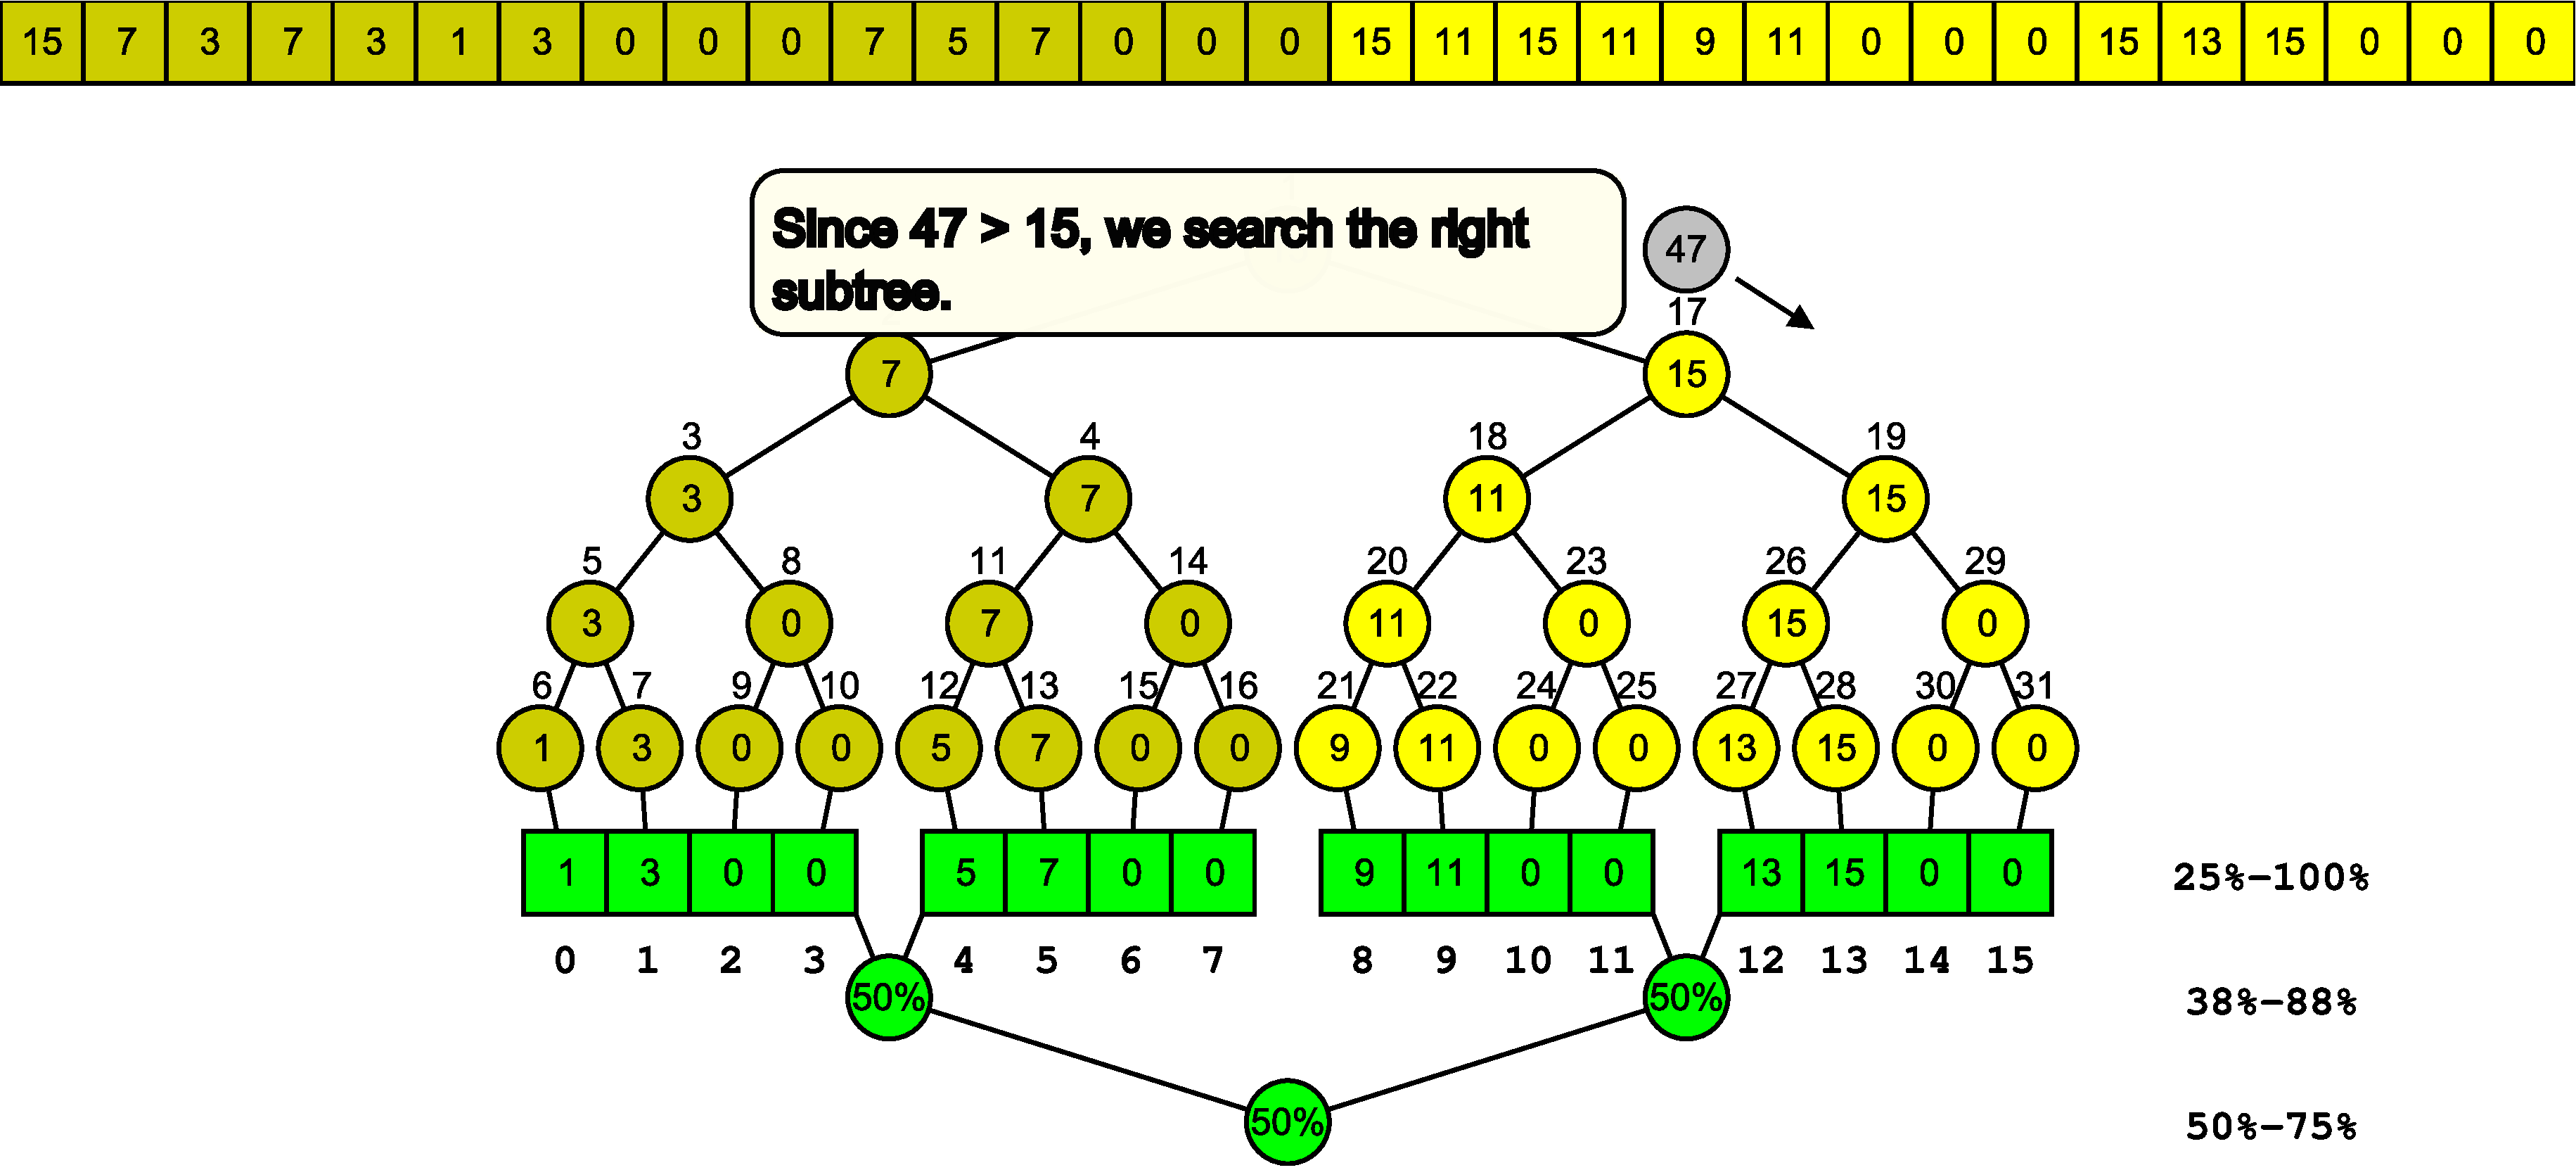
\includegraphics[width=0.8\textwidth]{figures/screenshots/2014-04-30_14-19-57.pdf}
%\end{figure}